\section{Sensitivity of LHC measurements to Vector-like Quarks}
\label{sec:VLQ}
Vector-like quarks belong to a separate family than the SM quarks. They are non-chiral, and thus both the left- and right-handed components transofrm the same way under the SM symmetries. This enables them to have a bare mass term and obtain mass without interacting with the Higg boson. Consequently, they are not constrained by Higgs measurements, unlike a fourth generation in the SM quark family. In short, VLQs are simplest example of coloured fermions still allowed by experimental data \cite{Aguilar_Saavedra_2013}. 

Vector-like quarks arise in many classes of BSM theories, such as composite Higgs that assume electroweak symmetry breaking is due to a a new strongly interacting sector~\cite{witzel2019review}, or little Higgs models that introduce extended global symmetries, or models with extra dimensional symmetries \todo{Add some citations for these models}. As with most models extending the SM, many of these introduce new sources of CP violation.

For the material presented in this section, vector-like quarks are studied in a model-independent fashion involving few free parameters. The framework is developed in Reference~\cite{}, which presents an effective Lagrangian description for vector-like quarks that is easily translated to experimental observables. The Lagrangian is written in equation 3.2 of Reference~\cite{} as:
\begin{equation}
  \label{eq:vlqlagr}
  \begin{split}
    \mathcal{L} =
    &  \kappa_B \left[
      \sqrt{\frac{\zeta_i\xi^{B}_{W}}{\Gamma^0_{W}}} \frac{g}{\sqrt{2}} [\bar{B}_{L/R} W^-_\mu \gamma^\mu u^i_{L/R}]
      +  \sqrt{\frac{\zeta_i\xi^{B}_{Z}}{\Gamma^0_{Z}}} \frac{g}{2c_W} [\bar{B}_{L/R} Z_\mu \gamma^\mu d^{\,i}_{L/R}]
      -  \sqrt{\frac{\zeta_i\xi^{B}_{H}}{\Gamma^0_{H}}} \frac{M_B}{v} [\bar{B}_{R/L} H d^{\,i}_{L/R}]
    \right] \\
    + &   \kappa_T \left[
      \sqrt{\frac{\zeta_i\xi^{T}_{W}}{\Gamma^0_{W}}} \frac{g}{\sqrt{2}} [\bar{T}_{L/R} W^+_\mu \gamma^\mu d^{\,i}_{L/R}]
      +  \sqrt{\frac{\zeta_i\xi^{T}_{Z}}{\Gamma^0_{Z}}} \frac{g}{2c_W} [\bar{T}_{L/R} Z_\mu \gamma^\mu u^i_{L/R}]
      -  \sqrt{\frac{\zeta_i\xi^{T}_{H}}{\Gamma^0_{H}}} \frac{M_T}{v} [\bar{T}_{R/L} H u^i_{L/R}]
    \right] \\
    +  &  \kappa_X \left[
      \sqrt{\frac{\zeta_i}{\Gamma^0_{W}}} \frac{g}{\sqrt{2}} [\bar{X}_{L/R} W^+_\mu \gamma^\mu u^i_{L/R}]
    \right]
    + \kappa_Y \left[
      \sqrt{\frac{\zeta_i}{\Gamma^0_{W}}} \frac{g}{\sqrt{2}} [\bar{Y}_{L/R} W^-_\mu \gamma^\mu d^{\,i}_{L/R}]
    \right] + \text{h.c.} \, ,
    % + & \kappa_g \left[ \frac{g_s v}{2\Lambda^2} f_i^{L/R} \bar{Q}_{R/L} G_{\mu\nu}\sigma^{\mu\nu} q^{i}_{L/R} \right] + h.c...
  \end{split}
\end{equation}
where $B$, $T$, $X$, and $Y$ are the four types of vector-like quarks with triplet colour charges, and electromagnetic charges $-\frac{1}{3}$, $\frac{2}{3}$, $\frac{5}{3}$ and $-\frac{4}{3}$ respectively. The couplings with the photon and gluon are derived via the standard gauge invariance route. The overall coupling strength of the vector-like quarks $Q$ are governed by the parameters $\kappa_Q$. $\zeta_i$ represents the coupling of the vector-like quarks to the $i^\text{th}$ generation SM quark. $\xi^B_V$ and $\xi^T_V$ govern the couplings of the $B$ and $T$ quarks to $Z$, $W$, and Higgs bosons via new $QqV$ vertices. Another free parameter is the mass of the new quarks, denoted as $M_Q$. Under the assumption that $\sum_{V} \xi^B_{V} = 1$ and $\sum_{V} \xi^T_{V} = 1$, and $\sum_{i} \zeta_i = 1$, the branching ratio of any vector-like quark to an SM quark and gauge boson is written as
\begin{equation}
    \textrm{BR}(Q \rightarrow Vq_i) = \zeta_i\xi^{V}.
\end{equation}


This combination of couplings means that the VLQs may be pair-produced from SM
initial states via the strong and EM interactions,
singly produced via the weak interaction, and weakly pair-produced by
$t$-channel exchange of an SM weak boson. They only decay via their weak
interaction, into the mixtures of SM weak bosons and quarks governed by the
$\xi$ and $\zeta$ parameters. Examples of leading-order Feynman diagrams for VLQ production are shown in
Figure~\ref{fig:feyndiags}.

\begin{figure}[t]
  \centering
  \subfloat[]{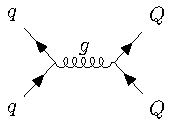
\includegraphics[]{feynmanDiagrams/diagram-5.pdf}\label{fig:feyndiags:QQ1}}
  \subfloat[]{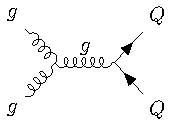
\includegraphics[]{feynmanDiagrams/diagram-9.pdf}\label{fig:feyndiags:QQ2}}
  \subfloat[]{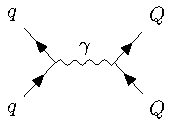
\includegraphics[]{feynmanDiagrams/diagram-6.pdf}\label{fig:feyndiags:QQ3}}\\
  \subfloat[]{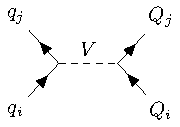
\includegraphics[]{feynmanDiagrams/diagram-8.pdf}\label{fig:feyndiags:QQ'1}}
  \subfloat[]{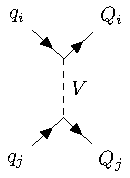
\includegraphics[]{feynmanDiagrams/diagram-7.pdf}\label{fig:feyndiags:QQ'2}}\\
  \subfloat[]{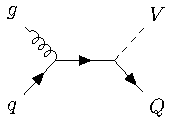
\includegraphics[]{feynmanDiagrams/diagram-1.pdf}\label{fig:feyndiags:QV1}}
  \subfloat[]{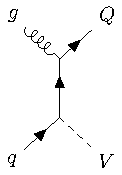
\includegraphics[]{feynmanDiagrams/diagram-2.pdf}\label{fig:feyndiags:QV2}}
  \subfloat[]{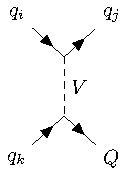
\includegraphics[]{feynmanDiagrams/diagram-3.pdf}\label{fig:feyndiags:Qq1}}
  \subfloat[]{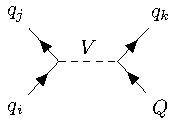
\includegraphics[]{feynmanDiagrams/diagram-4.pdf}\label{fig:feyndiags:Qq2}}
  \caption{Leading-order Feynman diagrams for production of VLQs $Q$.  The top row
  (\protect\subref*{fig:feyndiags:QQ1}--\protect\subref*{fig:feyndiags:QQ3}) shows VLQ
  pair-production diagrams via strong and EM interactions, which do not depend
  on $\kappa$.  The second row
  (\protect\subref*{fig:feyndiags:QQ'1}--\protect\subref*{fig:feyndiags:QQ'2}) shows
  pair-production of VLQs via a weak boson $V \in \{W,Z,H\}$, which may lead to
  different-flavoured VLQs in the final state.  The third row
  (\protect\subref*{fig:feyndiags:QV1}--\protect\subref*{fig:feyndiags:Qq2}) shows
  single-production of $Q$ in association with a weak boson or
  SM quark $q$.}
\label{fig:feyndiags}
\end{figure}

% Still, experimental searches assume that new quarks only couple to third generation SM quarks; though this is a natural expectation, mixings with lighter generations are not at all forbidden, and they can provide different signatures or affect the number of events in the final states tested by experiments, thus modifying current bounds.
\subsection{Phenomenology of VLQs}


\subsection{Comparison to \ATLAS searches}


\subsection{}